\chapter{Functions}
\section{Basics}
A function \emph{f}, from A to B is an assignment of exactly one element of B
to each element in A. \\
For example: Let \emph{f} be a function such that $\forall x \in \mathbb{R}$,
$f(x) = x^{2}$. You can observe that for any desired value of x, there is only
one unique mapping to $f(x)$. The reverse is not always true! \\ \\
A function is considered \textbf{\underline{one-to-one or injective}} if $f(x)
= f(y) \Leftrightarrow x = y$ \\ \\
A function from A to B is \textbf{\underline{onto or surjective}} if $\forall y
\in B$ $\exists x \in A$ such that $f(x) = y$. \\ \\
A function that is both one-to-one and onto is called a
\textbf{\underline{bijection}}. A function that is bijective implies that an
inverse for the function exists! \\ \\
\textsc{\underline{For Example:}} Consider the function $f:\mathbb{R}
\rightarrow \mathbb{R}$ such that $f(x) = 12x + 5$. Show that \emph{f} has an
inverse and find its inverse. \\
\indent \textbf{Solution:} First we have to show that f is injective. \\
\indent \indent Let us assume that $f(x_{1}) = f(x_{2})$.\\ \indent \indent
Then, $12x_{1} + 5 = 12x_{2} + 5 \Leftrightarrow 12x_{1} = 12{x2}
\Leftrightarrow x_{1} = x_{2}$. Thus, f is injective! \\
\indent Next, we have to show that f is surjective. \\
\indent \indent Let $f(x) = y$. Then, $y = 12x + 5$. \\
\indent \indent Then, $x = \frac{y - 5}{12}$. One can observe that for any real
number y, there exists a real number x such that $x = \frac{y - 5}{12}$. Thus,
f is surjective! \\
\indent Since f is a bijection, the inverse of f $f^{-1}(x) = \frac{x - 5}{12}$

\section{Floor and Ceiling Functions}
The \textbf{floor} of any real number returns the greatest integer that is less
than or equal to the real number. \\
The \textbf{ceiling} of any real number returns the smallest integer that is
greater than or equal to the real number. \\

For example: $\lfloor 2.5 \rfloor = 2$, $\lfloor -3.4 \rfloor = -4, \lfloor 7
\rfloor = 7$ \\
\indent \indent $\lceil 2.5 \rceil = 3, \lceil -3.4 \rceil = -3, \lceil \pi
\rceil = 4$.

\subsection{Proofs regarding Floor and ceiling functions}
I think it would be quite redundant to show proofs regarding floor and ceiling
functions. Questions that are similar to the ones shown in the
\href{http://nook.cs.ucdavis.edu/~koehl/Teaching/ECS20/Lectures/Lecture5_notes.pdf}{\underline{\emph{lecture
notes}}} generally show up on the midterms/final. Thus, I have omitted this one
topic as you can just read it up from the notes.

\section{Growth of Functions}
Often times, your task would be to determine the running time of an algorithm
that you just developed. These running times are represented as $O()$ (Big Oh),
$\Omega()$ (Big Omega), and $\Theta()$ (Big Theta) respectively.

\subsection{Big-O Notation}
The Big-O Notation is often used to represent the worst case analysis. Think of
Big-O as an upper bound for functions. The function f(x) is O(g(x)) if $[f(x)
\leq c \times g(x)]$ for all x > k, where c is a positive constant.\\
Let us consider an example: \\
Show that $x^{2} + 5x + 3$ is $O(x^{2})$ \\
\indent \emph{Solution:} In order for $x^{2} + 5x + 3$ to be $O(x^{2})$, $x^{2}
+ 5x + 3 \leq cx^{2}$. \\
\indent \indent We know that if $x > 1$ then, $5x \leq 5x^{2}$ and $3 \leq
3x^{2}$. \\
\indent \indent Adding these up we get: $x^{2} + 5x + 3 \leq x^{2} + 5x^{2} +
3x^{2} \leq 9x^{2}$. \\
\indent \indent Thus by selectively choosing $k = 1$ and $c = 9$, we can show
that $x^{2} + 5x + 3$ is $O(x^{2})$. \\ \\
\noindent For further verification and understanding, let us graph the
functions $x^{2} + 5x + 3$ and $9x^{2}$.

\begin{tikzpicture}
\begin{axis}[
    axis lines = left,
    xlabel = $x$,
    ylabel = {$f(x)$},
]
%Below the red parabola is defined
\addplot [
    domain=0:50,
    samples=100,
    color=red,
]
{x^2 + 5*x + 3};
\addlegendentry{$x^2 + 5x + 3$}
%Here the blue parabola is defined
\addplot [
    domain=0:50,
    samples=100,
    color=blue,
    ]
    {9*x^2};
\addlegendentry{$9x^{2}$}

\end{axis}
\end{tikzpicture} \\
As you can see, $x^2 + 5x + 3$ is never greater than $9x^{2}$.

\subsection{Big-Omega Notation}
The Big-Omega Notation is often used to represent the best case analysis. Think
of Big-Omega as an lower bound for functions. The function f(x) is
$\Omega(g(x))$ if $[f(x) \geq c \times g(x)]$ for all x > k, where c is a
positive constant.\\
Let us consider an example: \\
Show that $x^{3} + 6x^{2} + 3$ is $\Omega(x^{3})$ \\
\indent \emph{Solution:} In order for $x^{3} + 6x^{2} + 3$ to be
$\Omega(x^{3})$, $x^{3} + 6x^{2} + 3 \geq cx^{3}$. \\
\indent \indent We know that if $x > 1$ then, $x^{3} + 6x^{2} + 3 \geq x^{3}$.
\\
\indent \indent Thus by selectively choosing $k = 1$ and $c = 1$, we can show
that $x^{3} + 6x^{2} + 3$ is $\Omega(x^{3})$. \\ \\
\noindent For further verification and understanding, let us graph the
functions $x^{3} + 6x^{2} + 3$ and $x^{3}$.

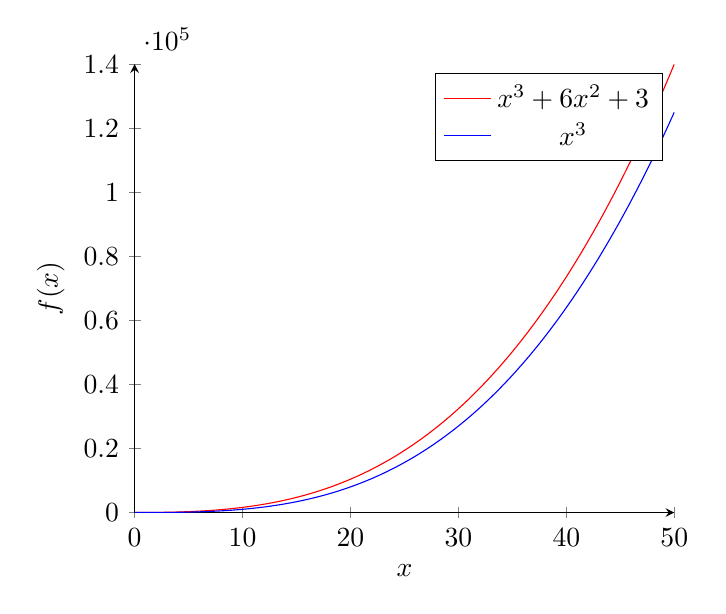
\begin{tikzpicture}
\begin{axis}[
    axis lines = left,
    xlabel = $x$,
    ylabel = {$f(x)$},
]
%Below the red parabola is defined
\addplot [
    domain=0:50,
    samples=100,
    color=red,
]
{x^3 + 6*x^2 + 3};
\addlegendentry{$x^{3} + 6x^{2} + 3$}
%Here the blue parabola is defined
\addplot [
    domain=0:50,
    samples=100,
    color=blue,
    ]
    {x^3};
\addlegendentry{$x^{3}$}

\end{axis}
\end{tikzpicture} \\
As you can see, $x^{3} + 6x^{2} + 3$ is always greater than $x^{3}$.
\subsection{Big-Theta Notation}
The Big-Theta Notation is often used to represent the average case analysis.
Think of Big-Theta as a tight bound for functions. The function f(x) is
$\Theta(g(x))$ if f(x) is $O(g(x))$ and if f(x) is $\Omega(g(x))$ \\
Let us consider an example: \\
Show that $x^{2} + 4x + 7$ is $\Theta(x^{2})$ \\
\indent \emph{Solution:} First, we have to show that $x^{2} + 4x + 7$ is
$O(x^{2})$. \\
\indent \indent Then, $x^{2} + 4x + 7 \leq cx^{2}$. \\
\indent \indent We know that for all $x > 1$, $4x \leq 4x^{2}$ and $7 \leq
7x^{2}$. Adding these up, we can say that $x^{2} + 4x + 7 \leq 12x^{2}$. Thus
by selectively choosing $k = 1$ and $c = 12$ we can conclude that $x^{2} + 4x +
7$ is $O(x^{2})$.\\
\noindent Next, we have to show the Big-Omega relation between these two
functions. \\
\indent \indent We know that for all $x > 1$ $x^{2} + 4x + 7 \geq x^{2}$
\indent \indent Thus by selectively choosing $k = 1$ and $c = 1$ we can
conclude that $x > 1$ $x^{2} + 4x + 7$ is $\Omega(x^{2})$. \\
\indent \indent Thus $\forall x > 1$ we can infer that:
\begin{center}
    $x^{2} \leq x^{2} + 4x + 7 \leq 12x^{2}$
\end{center}
\indent \indent Thus, $x^{2} + 4x + 7$ is $\Theta(x^{2})$
\subsection{Why do we need all this?}
Often times in algorithm analysis, you deal with large chunks of data. If, for
example, $n = 10$ where n is the number of elements, then it doesn't really
matter how good or bad our Big-Oh is. What if $n = 1,000,000$? Then $n^{2}$ and
$n^{3}$ would be significantly different. This is why we study the growth of
these functions. These notations are also sometimes referred to as time
complexities. You will learn about time complexities extensively in ECS 60 and
ECS 122A.
